\documentclass{article}
\usepackage{subcaption}
\usepackage{natbib}
\usepackage{tikz-feynman}

\begin{document}
\begin{figure*}[!t]

    \begin{subfigure}[t]{0.5\textwidth}
    \centering
        
        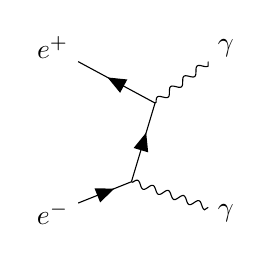
\begin{tikzpicture}
            \begin{feynman}
                \vertex (a) at (2.3, 0.5);
                \vertex (b) at (2.0, -0.5);
                \vertex (i1) at (1.0, 1.2) {$e^+$};
                \vertex (i2) at (1.0, -0.9) {$e^-$};
                \vertex (o1) at (3.2, 1.2) {$\gamma$};
                \vertex (o2) at (3.2, -0.9) {$\gamma$};

                \diagram*{
                    (i2) -- [fermion] (b) -- [fermion] (a) -- [fermion] (i1);
                    (a) -- [boson] (o1);
                    (b) -- [boson] (o2);
                };
            \end{feynman}
        \end{tikzpicture}
    \end{subfigure}
    \hspace{-2.0cm}
    \begin{subfigure}[t]{0.5\textwidth}
    \centering
        
        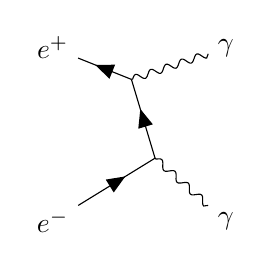
\begin{tikzpicture}
            \begin{feynman}
                \vertex (a) at (2.0, 0.8);
                \vertex (b) at (2.3, -0.2);
                \vertex (i1) at (1.0, 1.2) {$e^+$};
                \vertex (i2) at (1.0, -1.0) {$e^-$};
                \vertex (o1) at (3.2, 1.2) {$\gamma$};
                \vertex (o2) at (3.2, -1.0) {$\gamma$};

                \diagram*{
                    (i2) -- [fermion] (b) -- [fermion] (a) -- [fermion] (i1);
                    (a) -- [boson] (o1);
                    (b) -- [boson] (o2);
                };
            \end{feynman}
        \end{tikzpicture}
    \end{subfigure}

    \caption{Figure 1: Feynman graph for the lowest order contributions to electron position anihilation \cite{martin2017particle}.}

\end{figure*}

\bibliographystyle{plain}
\bibliography{references}
\end{document}
